\section{Evaluation}
\label{sec:evaluation}
\begin{figure}[t]
    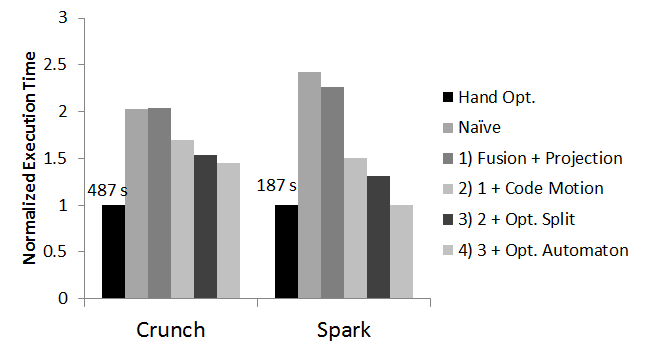
\includegraphics[width=8.6cm]{figures/word-count.png}
   \caption{Word Count benchmark.}
   \label{fig:word-count}%\vspace{10pt}
\end{figure}
We evaluate the optimizations by comparing the performance of three
programs:
\emph{i)} a word count with prior text processing, \emph{ii)} TPCH \cite{tpch}
query 12 and \emph{iii)} a k-means application. To evaluate the extensibility
of the framework we introduce a new \tool module that represents
vectors in the k-means benchmark.

All experiments were performed on the Amazon EC2 Cloud, using 20 "m1.large"
nodes as slaves and one as a master. They each have 7.5 GB of memory, 2 virtual
cores with 2 EC2 compute units each, 850 GB of instance storage distributed over
2 physical hard drives and they have a 1 Gb/s network interface. Prior to the
experiments we have measured up to 50 MB/s between two nodes. For the Hadoop
experiments we used the cdh3u4 Cloudera Hadoop distribution. On top of it we
used Crunch version 0.2.4. We used Whirr 0.7.1 \cite{whirr} to
set up the cluster, ensured that both hard drives were used for the
distributed file system and set the setting to reuse the JVM for
multiple map tasks.
For benchmarking Spark we used Spark version 0.5.0 for the tests, and
started the cluster using Spark's EC2 script.
For Spark we had to tweak settings to ensure that the programs run
correctly, including increasing the amount of available memory to 6 GB and
setting the parallelism to a value found after experimentation.

% Regular expressions
While doing preliminary benchmarking we found some simple optimizations focused
on regular expressions that we needed to include in \tool in order to have a fair
comparison against Pig, which contains them. We implemented a fast splitter,
which uses an efficient character comparison whenever the regular expression
allows this. Additionally, based on the regular expression pattern we select
between Java's implementation and the \emph{dk.brics.automaton} library \cite{mollerdk}.
% For a fairer comparison with Pig we adapted some of their regular expression
% optimizations for our program. Pig makes use of a faster library
% \cite{mollerdk} and implements an optimized splitting function when the
% regular expression becomes a simple comparison of one character. We
% implemented a frontend for regular expressions which automatically selects the
% best variant for each expression and operation.

% Data Serialization
For serialization of data we used \tool to generate specialized code to achieve minimal overhead for Crunch. 
For Spark we used the standard serialization mode which uses Kryo. All
benchmarks were run three times and in the figures we present the average
value. We also computed the standard deviations, but we omitted them since they
are smaller than 3\% in all the experiments.

We made the \tool code, as well as the generated code, available on
\url{https://github.com/jet-framework/jet}.


% WordCount
\subsection{Parsing and Word Count}
\label{subsec:parsing-word-count}

In this benchmark we evaluate the performance of \tool's compiler optimizations
without focusing on projection insertion. We chose a word count application
that, prior to the inexpensive network shuffle, parses the input with 5 regular
expressions making this job CPU bound. For this evaluation we start with an the
 na\"{\i}ve version of the program and add optimizations one by one. We first add
the operation fusion and projection insertion optimizations. We then include
code motion that removes regular expression compilation out of hot loops. Next
we add the fast splitter and for the fully optimized version we also use the
optimized automaton regular expression library.

Our input is a 124 GB set of plain text version of Freebase Wikipedia articles.
The program uses five regular expressions to remove words of the input that were
not parts of the plaintext in the article. This benchmark does not benefit from
projection insertion but we include it for the comparison
with the Pig framework in Section \ref{subsec:pig}.

In Figure \ref{fig:word-count} we show the job times for these versions
normalized to the hand-optimized program version. Compared to the na\"{\i}ve
version, the performance improvements of
all optimizations combined are from 40\% for Crunch
and 143\% for Spark. The base performance of the frameworks differ
by a large margin for this benchmark. In
Spark, we notice larger benefits from our optimizations. We argue that it has
significantly smaller IO overhead so that the optimizations have a bigger
impact. 

% TPCH q12
\subsection{TPCH Query 12}
\label{subsec:tpch-query-12}

This benchmark evaluates all optimizations combined but emphasizes the
projection insertion. We chose the TPCH query 12 which includes an expensive
\code{join} operation after which only two columns of the original data are
used, thus giving projection insertion opportunity to eliminate unused columns.
We evaluate all optimizations separately and all of them together and compare it
to the na\"{i}ve version. As the data set we use 200 GB plain text input
generated by the DbGen tool \cite{tpch}.

In Figure \ref{fig:tpch} we show job times for different optimizations
normalized to the original program version on different frameworks. We notice
that projection insertion gives 30\% percent better performance on Crunch while
on Spark the projection insertion improves the performance by 35\%. 

\todo{MORE!!!!}
% We believe that either network shuffle or the \code{join} operation are less
% optimal in Spark.
% In this benchmark the optimizations interact with each other. The absolute
% performance gain for combined optimizations is 3\% greater for Crunch, equal for
% Scoobi and 9\% smaller for Spark than the sum of the absolute individual gains.

\subsection{Comparison with Pig}
\label{subsec:pig}
\begin{figure}[t]
    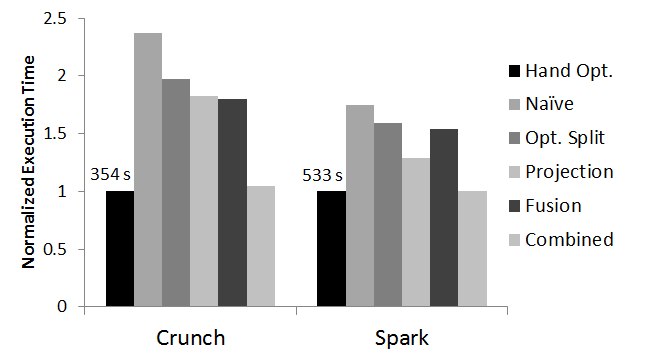
\includegraphics[width=8.6cm]{figures/tpch.png}
   \caption{TPCH query 12 benchmark.}
  \label{fig:tpch}%\vspace{10pt}    
\end{figure}
\begin{figure}[t]
    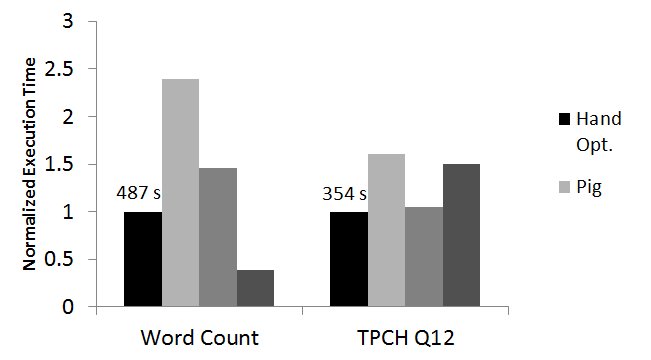
\includegraphics[width=8.6cm]{figures/pig.png}
   \caption{Comparison between Pig, Scoobi, Spark and Crunch.}
   \label{fig:pig}%\vspace{10pt}
\end{figure}

\begin{figure}[t]
    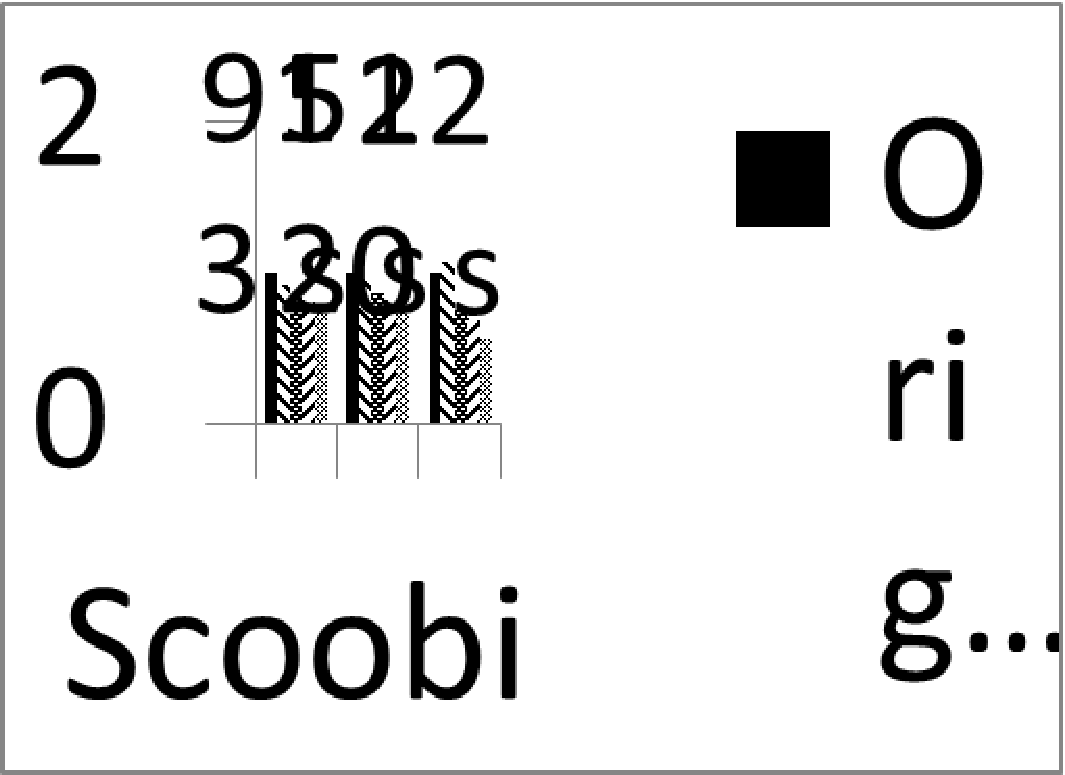
\includegraphics[width=8.6cm]{figures/k-means}
   \caption{K-means benchmark.}
   \label{fig:k-means}%\vspace{10pt}
\end{figure}

In Figure \ref{fig:pig} we com

% Pig Comparison
In Figure \ref{fig:pig} we compare the hand-optimized Hadoop and Pig programs
with our most optimized program versions.
The y-axis is normalized to the hand-optimized Hadoop and overall
job time is stated above the bar. 

We notice that our generated Crunch programs are faster than Pig by 53\% on
TPCH Q12 and 65\% on Wordcount. For the word count benchmark even the naive
version is faster than Pig by 18\%, we believe this to be due to the high
overhead of Pig's String operators. We further see that for TPCH Q12, the
performance of our program version is almost as fast as the hand-optimized
Hadoop version.

% Spark
For the sake of showing a comparison between the Hadoop based frameworks
and the Spark framework we include the Spark results in the graph. Spark
performs better for the word count example, and performs worse than Crunch in
the TPCH benchmark. We are uncertain about the exact causes of this behaviour.
However, code portability of \tool can be used to select the appropriate
execution engine for each program. 

\subsection{Extensibility}
\label{subsec:kmeans}

To evaluate the extensibility of \tool we decided to extend it in two ways: 
with a high-performance abstraction for the k-means benchmark and with a new
code generator that targets the Crunch framework.
 
\paragraph{Vector for k-means} 
% K-means language extensibility with KMeans
We took a version of Spark's k-means \cite{spark-nsdi} application and
ported it to \tool. This application can neither benefit from projection
insertion nor from operation fusion. The Spark code makes use of an abstraction
for multi-dimensional points called \code{Vector}, which uses iterators. We added
a Vector module to \tool which uses compiler support to generate efficient loops
instead of iterators. The implementation of the \code{Vector} module is 100
lines long and took one man day.

We evaluate the performance of our version against the original Spark version.
Because Spark is faster than Hadoop for iterative programs, we only evaluate
this benchmark on Spark.
As input we use synthetic data with 10 to 1000 dimensions, 100 centers and we keep the
$dimensions * points$ factor constant so that each input file is around 20 GB.

% Different backends
Our results are similar to those described by Murray et al. in
\cite{murray_steno:_2011}. In lower dimensions our optimization shows large
speedups while for 1000 dimensions our version performs slightly worse. We
believe that the iterator overhead is quite high in case of 10 dimensions, such
that our loops which removes it perform much better. At higher dimensions it is
possible that the JVM can do a better job optimizing if the code is smaller,
such that our pre-optimized and larger code becomes slightly slower. In any case
our implementation seems favorable as it performs more consistently for
different dimensions.

% Second addition

\paragraph{Crunch module}
Initially we planned to support Hadoop by generating code for the Scoobi
framework. We were unsatisfied by its performance however, which lead us to
implement code generation for the Crunch framework. The code for this module is
only 300 lines long and the implementation took four man days.
